
\section{广域互联网络的路由架构}

\subsection{广域网络的结构组成}

广域网是横跨国家、地区的、相互连接的全球性网络系统,如此庞大的体系决定了它必定将使用分布式的方式组成和管理,参加广域网络的组成部分依照一定的规则交换确认彼此的身份,并同时交换路由信息\citing{douzet2020measuring}。

\subsubsection{基本组成与管理方式}

互联网的基本组成单元是其中的成员网络,它们是能够被是作为一个行政实体的,一组或一个处于相同或类似策略管理下的路由器和终端设备,被称为自治系统(AS)。自治系统内部通过内部网关协定(IGP)交换系统内部的路由条目,而数以万计的自治系统相互独立建立自己的连接,并通过外部网关协定(EGP)在广域网层面交换彼此整个系统的路由项目,其中边界网关协定(BGP)是广域网络中唯一公认的外部网关协定\citing{rekhter2006border},因此后续的路由异常问题分析均以 BGP 协议为基础进行。

与通过 IP 地址确定设备的网络地址类似,BGP 协定使用一种称为自治系统编号的唯一标示符来确定一个自治系统的身份,它的范围是4个字节(0-4294967295)\citing{rekhter2006border}。在互联网中,互联网号码分配局(IANA)负责管理这些号码及所属于这些自治系统的 IP 地址的的分配,它通过一种层次结构将这些资源分配给五个区域互联网注册局(RIR),而这些注册局则通过本地互联网注册局(LIR)向下分配获取的资源和网络号码\citing{angieri2019distributed}。

\subsubsection{商业网络的层次结构}

在互联网中,路由信息的传递并不一定是无方向的。在实际的互联网络中,大部分具有较多直接连接或具有更优质线路的网络是商业公司,它们将向具有更低连接性的网络及其客户网络提供付费的连接服务,这直接体现在了路由信息的传递上,在与网络路由相关的研究中,这类单向的信息传递通常被称为非对等互联(Transit)\citing{gregori2011bgp}。

由于上述原因,互联网的路由结构从最初设计的完全分布式逐渐地转变为了具有了一定层次和中心性的结构\citing{vanbever2009hierarchical}:一些网络能够经由更少的自治系统,从而抵达互联网的每一个角落,它们被认为具有更高的中心度。

因而,有研究提出了“客户锥形”的概念\citing{luckie2013relationships}:一个自治系统的客户锥形是它自身和在广域网中能够观察到的通过非对等互联路由可以到达的所有AS,即它和它的任意阶客户。

% 来个公式

对于一个自治系统而言,位于它的客户锥形中的自治系统的路由一般会直接或间接地经由它,因而这项指标展示了它对网络资源的控制能力\citing{luckie2013relationships},即能够影响到网络中的哪些部分的路由。在一些研究中,它的大小常常被用作一种衡量标准,用于度量自治系统的相对规模\citing{doverspike2010structural}。

与此同时,一些网络常常还会与其它网络建立互利且双向的路由交换,相互直接交换各自的路由信息,通常任何一方都不向对方支付费用,这种关系被称为对等互联(Peering),通常这类对等路由不会继续发送给对等方以外的自治系统。\citing{vanbever2009hierarchical} \citing{luckie2013relationships} 在一些被称作互联网交换点的设施内,会有大量 AS 形成近似于全连接(Full Mesh)的对等互联关系,据调查显示,对等互联大大降低了流量结算成本,并降低了互联网日益提升的中心度\citing{luckie2013relationships}。

\begin{figure}[h]
    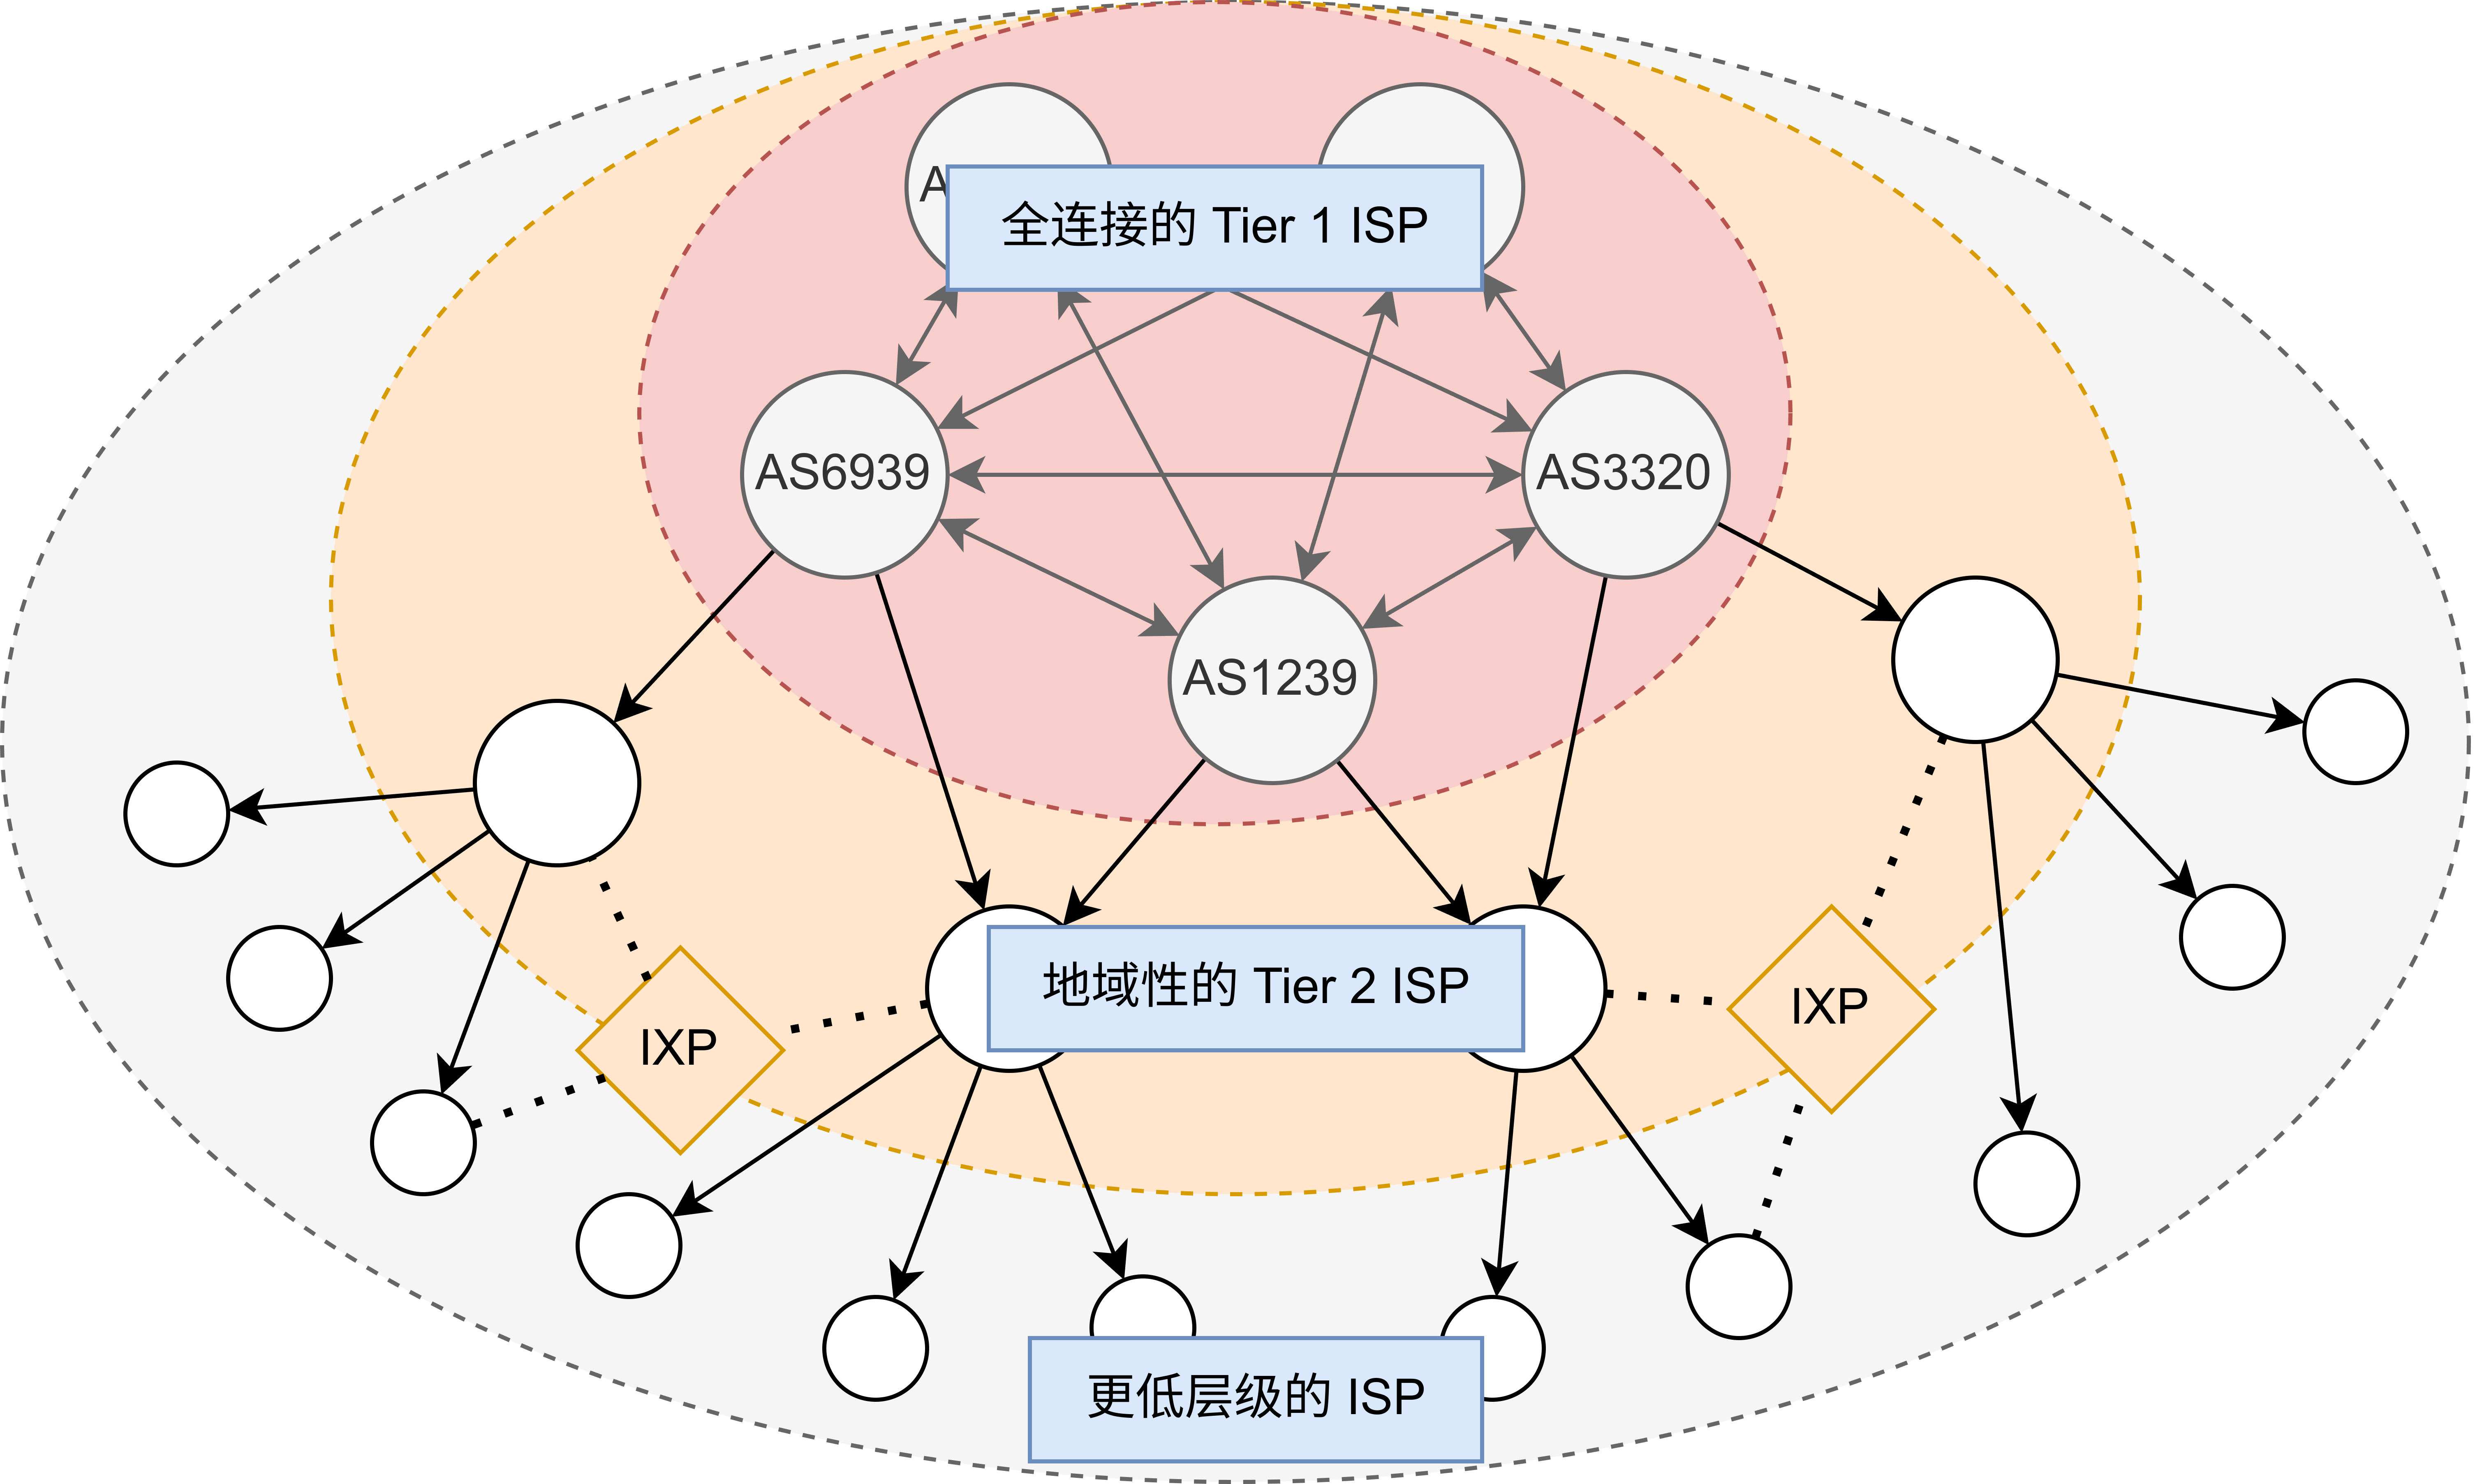
\includegraphics[width=0.7\linewidth]{chapter/c2_images/c2_wan-asn-structure.png}
    \caption{广域网络的层次结构}
    \label{c2_wan-asn-structure}
\end{figure}

图 \ref{c2_wan-asn-structure} 更加直观地展示了互联网中存在的三级层次结构\citing{doverspike2010structural}:彼此相互全连接(Full-Mesh)提供非对等互联路由(事实上即是全部网络路由)的I类自治系统(Tier 1);直接由I类自治系统提供非对等互联路由的II类自治系统(Tier 2);间接通过上级自治系统访问全部网络的III类自治系统(Tier 3);这些自治系统还直接或通过互联网交换点间接进行对等路由的交换。

\subsubsection{分布式网络的对等结构}

在互联网之外,还存在一些社区维护的实验性分布式网络\citing{mirz2018distributed},它们的大部分网络通常是双向提供非对等互联服务的,即在对等互联会话中交换全部已知路由,因此在结构上具有截然不同的特点,例如由于不存在商业关系,整体上具有更少的中心度、成员自治系统的组织一般不具有层次性。

中国教育和科研计算机网(China Education and Research Network,简称 CERNET)\citing{li2011china}是我国教育部、赛尔网络与众多国内高校合办的实验性网络。虽然 CERNET 本身是互联网的参与方,但它的成员单位大多拥有自己的自治系统号码,并相互通过 BGP 协议交换自身的路由,因而在内部能够被视作为一个分布式广域网络。

DN42(Decentralized Network 42)\citing{dn42us}是一个由社区发起的的去中心化网络。 与一般的网络不同的是,DN42 拥有着与其他网络相独立的地址空间、自治系统编号规则和域名系统,因此其架构完全独立于互联网,并且其参与方通常使用重叠网络(Overlay Network)技术,通过底层网络建立网络隧道与其它自治系统相互连接,而非借助光纤或网线的方式通过物理介质连接,这样的组网方式降低了网络的申请门槛,因而在尺度上具有一定的规模,适合用作网络相关研究。

\subsection{广域网络中的路由协议原理}

由于 BGP 协议在自治系统间的广泛性和通用性,广域网络中的路由在通常情况下指使用 BGP 协议在广域网中交换的路由,它与内部路由协议不同,不使用常见的最短路算法,而是让每一个自治系统保留一份当前视角的全球路由表,并直接根据路由表中的属性选择路由\citing{rekhter2006border}。以下将介绍它的基本原理。

\subsubsection{路由信息交换}

由于广域网的分布式和开放性,使得它的路由不存在用于统一调度和管理的中心机构,这使得它具有强大的纠错能力。即使自治系统之间没有直接连接,或是直接连接因故断开,边界路由协定会帮助路由器寻找替代路径,虽然可能在传输延迟、带宽等受到限制,但是仍然能够正常通信\citing{verma2018analysis}。总的来说,互联网的分布式系统理论上是具有良好的鲁棒性的。

自治域内通过内部路由协定交换的域内路由通常不会传播到自治域外,并且具有更少的层次结构,而由于处于统一管理之下,网络拓扑结构上的变化是可预测的,因而此类路由一般不会出现异常。而每个自治域之间的路由则由自治域间的链路状况、主机状况,甚至是政府的监管审查、贸易壁垒等非技术因素而决定,所有自治域共同组成分布式系统,互联网这一整体将随着各节点的情况改变而不断改变自身的拓扑结构,位于自治域之间的、通过边界路由协定交换的域间路由也将随之变化\citing{al2016bgp}。因为其路由条目属性过多、路由选择策略较为复杂,常常因为外界因素出现异常状况。

\subsubsection{路由选择算法}

与统一管理的内部路由协议不同,为了保证路由系统的所有参与者都能够自行决定最优路径,BGP 协议要求路由条目中的属性信息尽可能地能携带自定义的字段,并被任意途径的自治系统说采用。

% 总的来说,它包含四种类型的属性信息:

% \begin{enumerate}
%     \item 众所周知的强制属性:所有自治系统的路由器都能识别并处理,并且字段必须被包括在传递的每一条路由信息中。
%     \item 众所周知的可选属性:所有自治系统的路由器都能识别并处理,字段能够可选地被包括在传递的路由信息中。
%     \item 可选的传递性信息:能够被一些自治系统的路由器识别并处理,即使不能识别,也需要被包括在进一步转递出去的路由信息中。
%     \item 可选的非传递性信息:能够被一些自治系统的路由器识别并处理,它们能够被忽略掉,不被包括在进一步转递出去的路由信息中。
% \end{enumerate}

以下是协议中最常见的两种属性信息,它们将在后续章节的研究中使用:

\begin{enumerate}
    \item 自治系统路径(AS Path)\citing{rekhter2006border}是一种强制编码在路由条目中的信息,它表达了路由在自治系统层面的传递信息,可以被理解为一条由节点 ID(自治系统编号)组成的有向路径。每个自治系统在将路由信息转递前,都会在此路径的首部添加自己的AS号码,以防止路由循环。
    \item 社区(Community)\citing{donnet2008bgp}是一类可选的信息,它能够理解为这条路径所关联的标签,这类标签信息既可以是私有的(只在某些自治系统有效)也可以是共有的(一些预定义的属性会在所有自治系统生效),路由消息在传递的时候,自治系统的路由器能够根据规则去添加、删除和改写这些标签。
\end{enumerate}

与内部网关协定中复杂的权重不同,由于自治系统之间难以统一协调,加之过于巨大的网络拓扑使得精确的路径寻找较为困难,一般情形而言,广域网的 BGP 协议寻路使用最短自治系统路径,同时使用社区属性对一些需要特殊优先级的路由进行调整。

自治系统路径能够反映出路由中的拓扑信息,而社区属性是对整个路径的标签信息,通过这两个信息能够构建出一个有向带权重的图。由于其它信息在不同自治系统下具有不同的数值定义,因而无法仅通过数据集确定意义,故无参考价值,本文不再介绍。

